\section{Automatic Faults Detection of Photovoltaic Farms: solAIr, 
a Deep Learning-Based System for Thermal Images}

%1
\begin{frame}
    \frametitle{\textit{Automatic Faults Detection of Photovoltaic Farms: solAIr, 
a Deep Learning-Based System for Thermal Images}
    ~~------~~ Overview}

    In this paper, the authors develop a new DNN-based solar panel failure
    detection system.

    \colorbox{orange}{Highlights:}
    \begin{itemize}
        \item The database is obtained by UAVs equipped with a thermal infrared
            camera.
        \item Use the Mask RCNN as the main algorithm for the object detection
            and instance segmentation.
        \item The performance of proposed network and other mature network are
            compared.
    \end{itemize}

    \colorbox{orange}{Notes:} 

    The thermal images has many advantages than RGB images. However, 
    a normalization and a transformation into a black and white image
    are required, for obtaining a single information channel.


\end{frame}

%2
\begin{frame}
    \frametitle{\textit{Automatic Faults Detection of Photovoltaic Farms: solAIr, 
a Deep Learning-Based System for Thermal Images}
    ~~------~~ Mask RCNN}
    \begin{block}{Main task}
        The Mask RCNN can accomplish 3 tasks at the same time:
    \end{block}
    \begin{itemize}
        \item Location: It can give the boundary box of the object.
        \item Classification: The object classes are labeled.
        \item Segmentation: it segment the object at the instance level.
    \end{itemize}
    \begin{figure}[H]
        \centering
        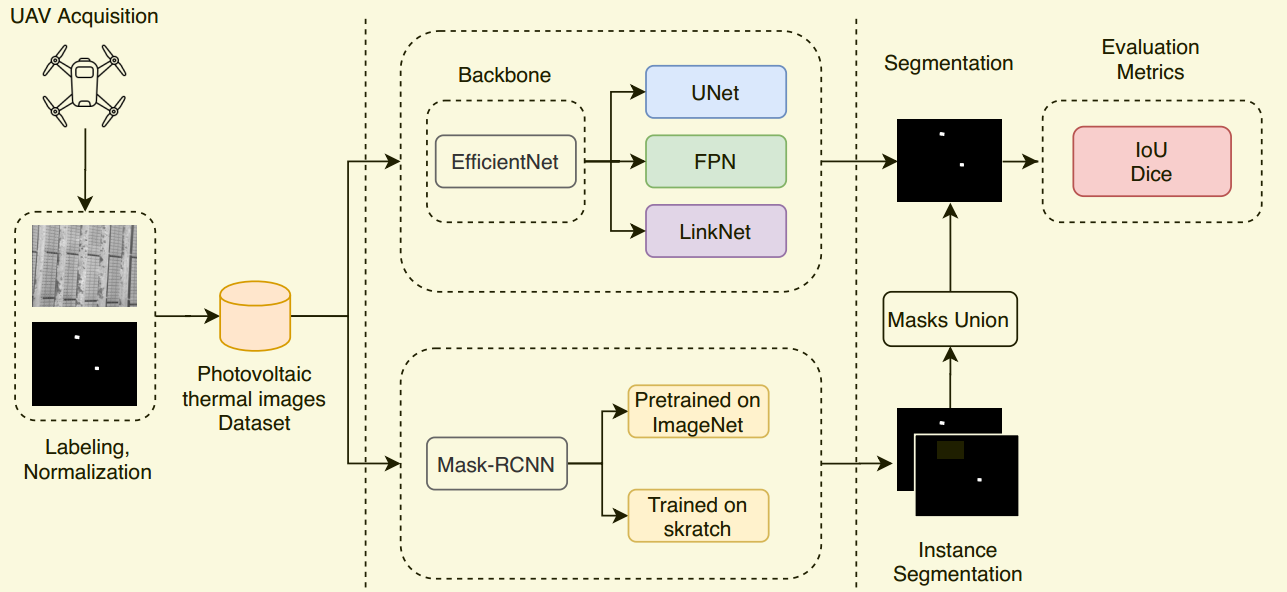
\includegraphics[width=0.8\textwidth]{./imgs/maask_rcnn}
    \end{figure}
\end{frame}
